%% -*- master.tex -*-

%% Copyright (C) 2012 - Ajit Pawar

% Use memoir documentclass
\documentclass[a4paper, 11pt, article, oneside, final]{memoir}
\usepackage[breaklinks=true]{hyperref}
\usepackage[utf8]{inputenc}
\usepackage[T1]{fontenc}
\usepackage[english]{babel}

% Graphics
\usepackage{graphicx}
%\usepackage{subfig}

% Lets you comment out blocks of LaTeX code (i.e. avoid using %%) by simply
% writing \begin{comment} ... \end{comment}
\usepackage{verbatim}

% Fonts
\usepackage[sc]{mathpazo}
\linespread{1.05}         % Palatino needs more leading (space between lines)
\usepackage[T1]{fontenc}

% Fixme
\usepackage[footnote,draft,silent,nomargin]{fixme}

% Itemize
\renewcommand{\labelitemi}{$\ast$}

% Math
\usepackage{amsmath, amssymb, bm, mathtools, float}

% PDF include
\usepackage{pdfpages}

% Table of Content
\setcounter{secnumdepth}{3}
\setcounter{tocdepth}{3}

% Tables
\usepackage{longtable}

% URLs
\usepackage{url}

% BibTeX
\usepackage[square]{natbib}

\pagestyle{companion}

% Start document
\title{Course Name}

%% Ugly hack for adding a project name header
\author{
  {\noindent\HUGE\bfseries Project Name} \\ \\ \\
  John Doe, john@doe.com \\
  Jane Doe, jane@doe.com \\
}
\date{\today}

\begin{document}\sloppy
\maketitle

\newpage
\tableofcontents
\cleardoublepage

%% --*-- index.tex --*--

%% --*-- introduction.tex --*--

\begin{frame}{Introduction}
\framesubtitle{Subtitle?}
Interesting pitch.
\end{frame}

%% end-of-introduction.tex

%% --*-- implementation.tex --*--

\chapter{Implementation}

Lorem ipsum dolor sit amet, consectetur adipisicing elit, sed do eiusmod tempor
incididunt ut labore et dolore magna aliqua. Ut enim ad minim veniam, quis
nostrud exercitation ullamco laboris nisi ut aliquip ex ea commodo
consequat. Duis aute irure dolor in reprehenderit in voluptate velit esse cillum
dolore eu fugiat nulla pariatur. Excepteur sint occaecat cupidatat non proident,
sunt in culpa qui officia deserunt mollit anim id est laborum.

Random reference~\cite{FOO}.

A Figure.
\begin{figure*}[ht]
  \centering
  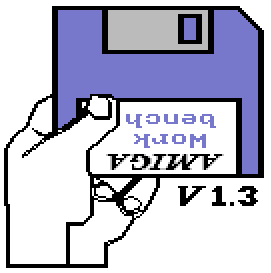
\includegraphics[width=0.5\textwidth]{images/figure.png}
  \caption{A fancy figure}
  \label{img:figureName}
\end{figure*}

%% end-of-implementation.tex

%% --*-- discussion.tex --*--

\chapter{Discussion}

Lorem ipsum dolor sit amet, consectetur adipisicing elit, sed do eiusmod tempor
incididunt ut labore et dolore magna aliqua. Ut enim ad minim veniam, quis
nostrud exercitation ullamco laboris nisi ut aliquip ex ea commodo
consequat. Duis aute irure dolor in reprehenderit in voluptate velit esse cillum
dolore eu fugiat nulla pariatur. Excepteur sint occaecat cupidatat non proident,
sunt in culpa qui officia deserunt mollit anim id est laborum.

%% end-of-discussion.tex

%% --*-- conclusion.tex --*--

\chapter{Conclusion}

Lorem ipsum dolor sit amet, consectetur adipisicing elit, sed do eiusmod tempor
incididunt ut labore et dolore magna aliqua. Ut enim ad minim veniam, quis
nostrud exercitation ullamco laboris nisi ut aliquip ex ea commodo
consequat. Duis aute irure dolor in reprehenderit in voluptate velit esse cillum
dolore eu fugiat nulla pariatur. Excepteur sint occaecat cupidatat non proident,
sunt in culpa qui officia deserunt mollit anim id est laborum.

%% end-of-conclusion.tex


%% end-of-index.tex


\newpage

\bibliographystyle{plainnat}
\bibliography{reference}

\newpage
\appendix
%% --*-- index.tex --*--

%% --*-- introduction.tex --*--

\begin{frame}{Introduction}
\framesubtitle{Subtitle?}
Interesting pitch.
\end{frame}

%% end-of-introduction.tex

%% --*-- implementation.tex --*--

\chapter{Implementation}

Lorem ipsum dolor sit amet, consectetur adipisicing elit, sed do eiusmod tempor
incididunt ut labore et dolore magna aliqua. Ut enim ad minim veniam, quis
nostrud exercitation ullamco laboris nisi ut aliquip ex ea commodo
consequat. Duis aute irure dolor in reprehenderit in voluptate velit esse cillum
dolore eu fugiat nulla pariatur. Excepteur sint occaecat cupidatat non proident,
sunt in culpa qui officia deserunt mollit anim id est laborum.

Random reference~\cite{FOO}.

A Figure.
\begin{figure*}[ht]
  \centering
  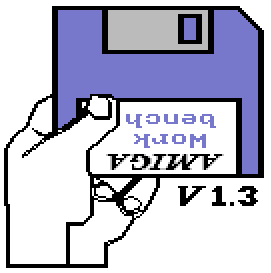
\includegraphics[width=0.5\textwidth]{images/figure.png}
  \caption{A fancy figure}
  \label{img:figureName}
\end{figure*}

%% end-of-implementation.tex

%% --*-- discussion.tex --*--

\chapter{Discussion}

Lorem ipsum dolor sit amet, consectetur adipisicing elit, sed do eiusmod tempor
incididunt ut labore et dolore magna aliqua. Ut enim ad minim veniam, quis
nostrud exercitation ullamco laboris nisi ut aliquip ex ea commodo
consequat. Duis aute irure dolor in reprehenderit in voluptate velit esse cillum
dolore eu fugiat nulla pariatur. Excepteur sint occaecat cupidatat non proident,
sunt in culpa qui officia deserunt mollit anim id est laborum.

%% end-of-discussion.tex

%% --*-- conclusion.tex --*--

\chapter{Conclusion}

Lorem ipsum dolor sit amet, consectetur adipisicing elit, sed do eiusmod tempor
incididunt ut labore et dolore magna aliqua. Ut enim ad minim veniam, quis
nostrud exercitation ullamco laboris nisi ut aliquip ex ea commodo
consequat. Duis aute irure dolor in reprehenderit in voluptate velit esse cillum
dolore eu fugiat nulla pariatur. Excepteur sint occaecat cupidatat non proident,
sunt in culpa qui officia deserunt mollit anim id est laborum.

%% end-of-conclusion.tex


%% end-of-index.tex


\end{document}

%% end-of-master.tex
